\documentclass[12pt]{article}
\usepackage[utf8]{inputenc}
\usepackage{graphicx}
\usepackage[a4paper,width=150mm,top=25mm,bottom=25mm]{geometry}

\title{
{
\includegraphics[width=4.5cm, height=3cm]{img/CSLogo.jpg}

\includegraphics[width=3cm, height=2.5cm]{img/MSALogo.jpg}}
\\
{Software Design Document for project ------------}
}



\author{Ahmed Mohamed,.... \\ Supervised by: Dr. ......}

\begin{document}

\maketitle

\section{Introduction}
\subsection{Purpose}
Identify the purpose of this SDD and its intended audience. (e.g. This software design
document describes the architecture and system design of XX.. ).


\subsection{Scope}
Provide a description and scope of the software and explain the goals, objectives and benefits
of your project. This will provide the basis for the brief description of your product.


\subsection{Overview}
Provide an overview of this document and its organization.



\subsection{Reference Material}
This section is optional.
List any documents, if any, which were used as sources of information for the test plan. 


\subsection{Definitions and Acronyms}
This section is optional.
Provide  definitions of all terms, acronyms, and  abbreviations that might exist to  properly 
interpret the SDD. These definitions should be items used in the SDD that are most likely not 
known to the audience.

\begin{table}[h]
\begin{tabular}{|l|l|}
\hline
\multicolumn{1}{|c|}{\textbf{Term}} & \multicolumn{1}{c|}{\textbf{Definition}}                                                                                              \\ \hline
Software Design Document (SDD)      & \begin{tabular}[c]{@{}l@{}}Used as the primary medium for communicating software \\ design information.\end{tabular}                  \\ \hline
Design Entity                       & \begin{tabular}[c]{@{}l@{}}An element of a design that is structurally and functionally \\ distinct from other elements.\end{tabular} \\ \hline
\end{tabular}
\end{table}

\section{System Overview}
Give a general description of the functionality, context and design of your project. Provide any 
background information if necessary.

\section{System Architecture}
\subsection{Architectural Design}
Develop a modular program structure and explain the relationships between the modules to 
achieve  the  complete  functionality of the  system. This is a  high level overview  of how responsibilities of the system were partitioned and then assigned to subsystems. Identify each 
high level subsystem and  the  roles or responsibilities assigned to it. Describe  how  these subsystems collaborate with each other in order to achieve the desired functionality. Don t go 
into too much detail about the individual subsystems. The main purpose is to gain a general understanding  of how  and why the system was decomposed, and  how the  individual parts
work together. Provide a diagram showing the major subsystems and data repositories and their interconnections. Describe the diagram if required.


\begin{figure}[tbh]
\centering
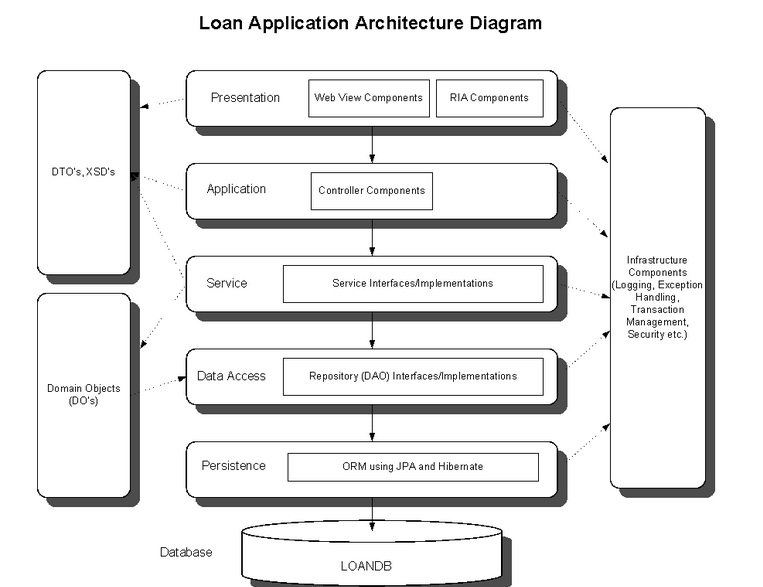
\includegraphics[width=0.7\linewidth]{./img/image}
\caption{Architectural Design}
\label{fig:image}
\end{figure}


\subsection{Decomposition Description}
Provide a decomposition of the subsystems in the architectural design. Supplement with text 
as needed. You may choose to give a functional description or an object oriented description. For a  functional description, put top level data  flow  diagram (DFD)  and  structural 
decomposition  diagrams. For an OO description, put subsystem model, object diagrams, generalization hierarchy diagram(s) (if any), aggregation hierarchy diagram(s) (if any),
interface specifications, and sequence diagrams here.


\subsection{Design Rationale}
Discuss the rationale for selecting the architecture described in 3.1 including critical issues
and  trade/offs that were  considered. You  may discuss other  architectures that were 
considered, provided that you explain why you didn't choose them.


\section{Data Design}
\subsection{Data Description}
Explain how the information domain of your system is transformed into data structures. Describe how the major data or system entities are stored, processed and organized. List any 
databases or data storage items.

\subsection {Data Dictionary}
Alphabetically list the system entities or major data along with their types and descriptions. If
you  provided  a  functional description  in  Section 3.2, list all the  functions and function 
parameters. If you provided an OO description, list the objects and its attributes, methods and 
method parameters.

\section{Component Design}
In this section, we take a closer look at what each component does in a more systematic way. If you gave a functional description in section 3.2, provide a summary of your algorithm for each 
function listed in 3.2 in procedural description language (PDL) or pseudo-code. If you gave an 
OO description, summarize each object member function for all the objects listed in 3.2 in PDL
or pseudo code. Describe any local data when necessary.


\section{Human Interface Design}

\subsection {Overview of User Interface}
Describe the functionality of the system from the user s perspective. Explain  how the user 
will be  able  to use  your system to complete  al the  expected  features and  the  feedback 
information that will be displayed for the user.

\subsection {Screen Images}
Display screenshots showing the interface from the users perspective. These can be  hand drawn
or you can use an automated drawing tool. Just make them as accurate as possible.



\subsection {Screen Objects and Actions}
A discussion of screen objects and actions associated with those objects.


\section{Requirements Matrix}
Provide a cross reference that traces components and data structures to the requirements in your
SRS document.
Use  a  tabular  format to show  which system  components satisfy each of the  functional 
requirements from the SRS. Refer to the functional requirements by the numbers/codes that you 
gave them in the SRS.


\section{APPENDICES}
This section is optional.
Appendices may be included, either directly or by reference, to provide supporting details that could 
aid in the understanding of the Software Design Document.

\section {References}
\bibliographystyle{IEEEtranS}

\bibliography{bab/dissertationbib}

\end{document}
